\documentclass[10pt]{article}
\usepackage[letterpaper,margin=0.9in]{geometry}
\usepackage{lmodern}
\usepackage[T1]{fontenc}
\usepackage{amsmath}
\usepackage{graphicx}
\usepackage{booktabs}
\usepackage{array}
\usepackage{longtable}
\usepackage{siunitx}
\usepackage{xcolor}
\usepackage{caption}
\usepackage{enumitem}
\usepackage{float}
\usepackage[colorlinks=true,linkcolor=black!70!blue,urlcolor=black!70!blue,citecolor=black!70!blue]{hyperref}
\captionsetup{font=small,labelfont=bf}
\setlist{nosep,leftmargin=1.4em}
\sisetup{detect-all}
\newcommand{\BaseInnerAt}{331}
\newcommand{\BaseOuterAt}{210}
\newcommand{\ZeroInnerAt}{326}
\newcommand{\ZeroOuterAt}{207}
\newcommand{\AtChangePct}{-1.3}
\newcommand{\BaseI}{1.27}
\newcommand{\ZeroI}{2.25}
\newcommand{\BaseP}{5.1}
\newcommand{\ZeroP}{10.0}
\newcommand{\BaseV}{4.03}
\newcommand{\ZeroV}{4.46}
\newcommand{\BaseT}{61}
\newcommand{\ZeroT}{95}
\newcommand{\WorstCoreB}{0.74}
\newcommand{\WorstCoreDesc}{0.750~in core, 0.875~in spacer}
\newcommand{\BaseShaftB}{0.46}
\newcommand{\StoredEnergyMJ}{66}
\newcommand{\LinVsNLPct}{+1.2}
\newcommand{\NRuns}{25}
\newcommand{\OuterODChangePct}{-0.4}
\newcommand{\OuterODInnerChangePct}{-0.4}

% \input inside a tabular leaves the following \bottomrule "misplaced";
% the primitive file read does not.
\makeatletter\newcommand\tabinput[1]{\@@input #1 }\makeatother

\title{\textbf{BPL-700 Magnet Circuit}\\[2pt]\large Spacer height sweep, coil geometry, and power-supply requirements}
\author{Marlow Nedelchev}
\date{\today}

\begin{document}
\maketitle


\begin{figure}[H]
\centering
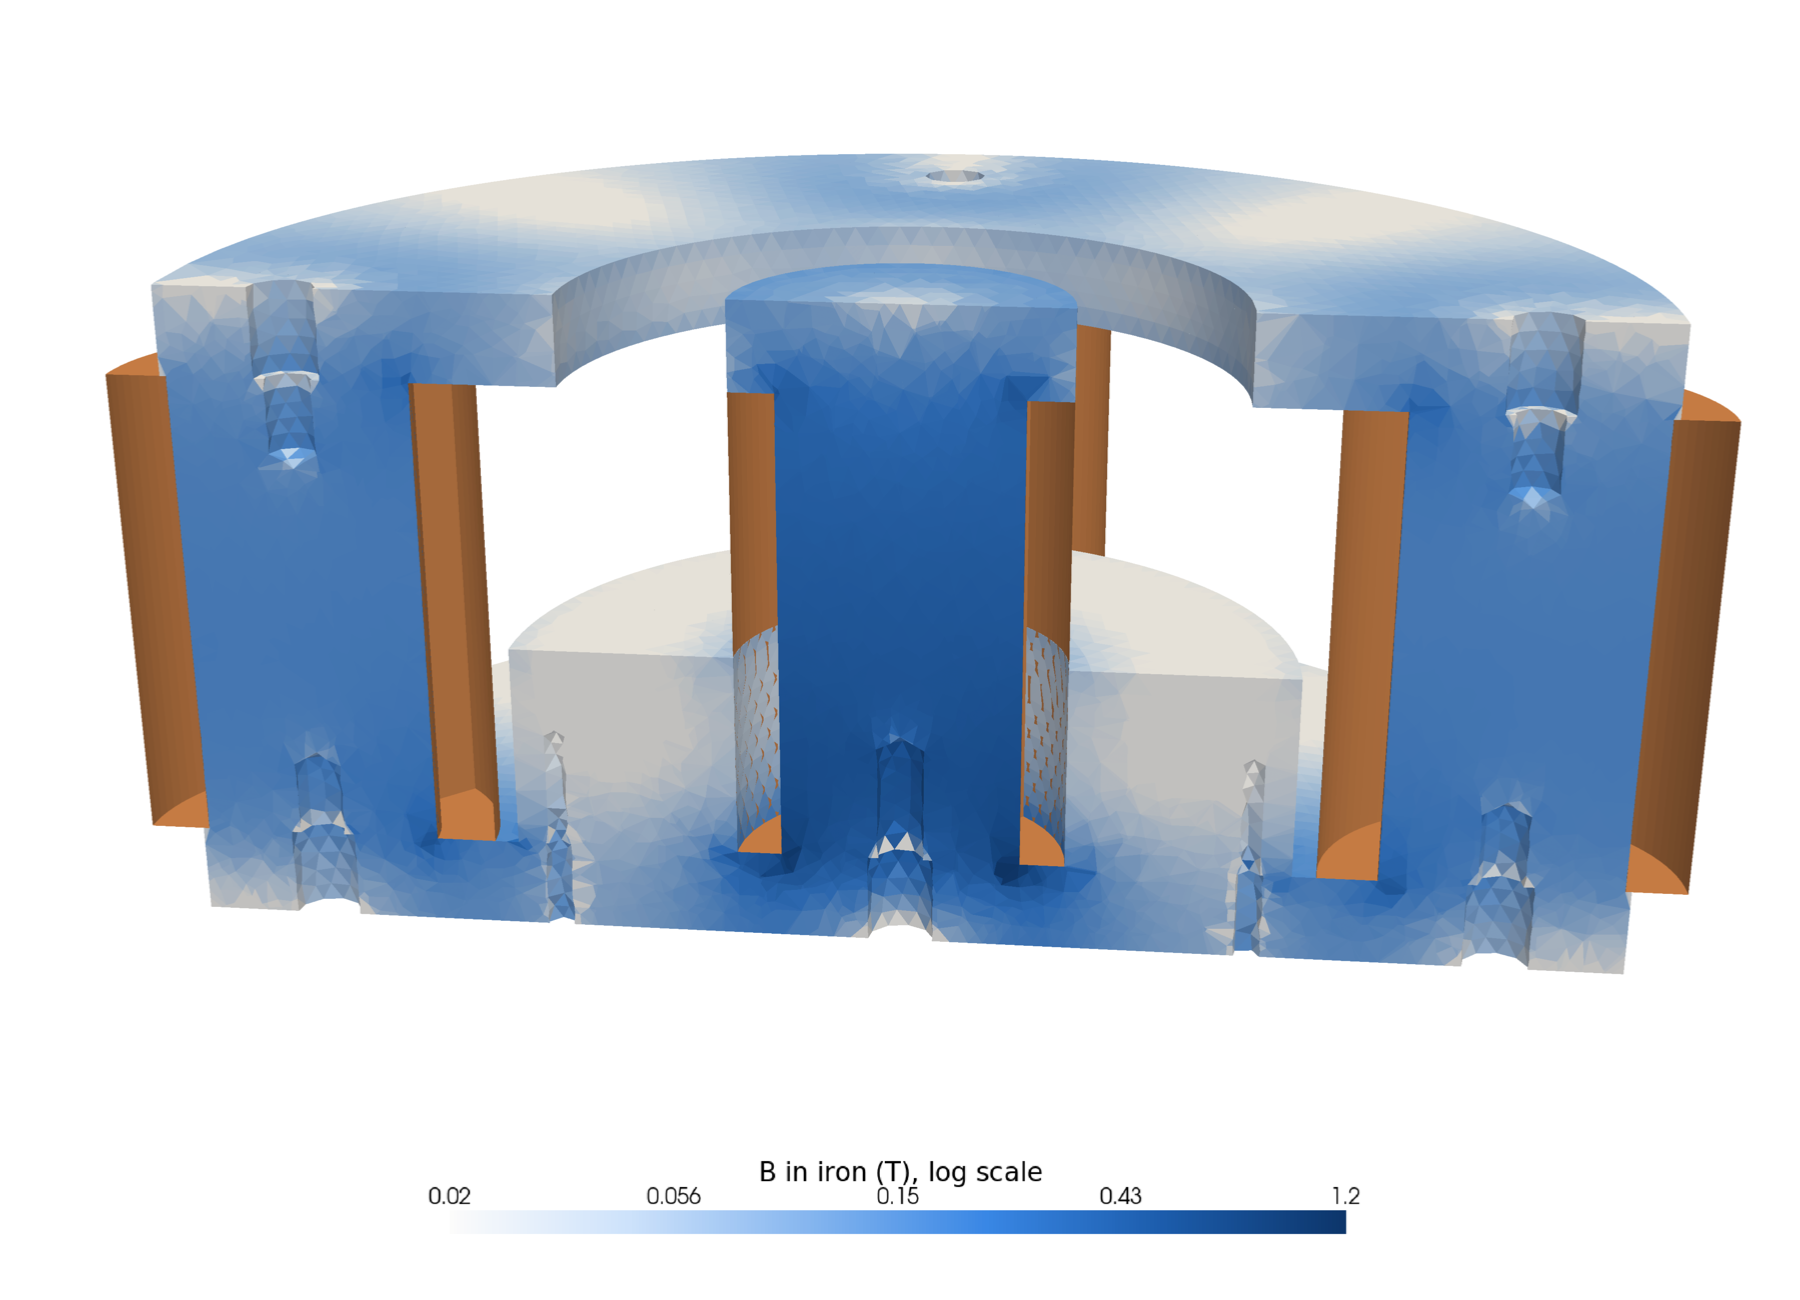
\includegraphics[width=0.78\linewidth]{figures/render_3d.png}
\caption{BPL-700 magnet circuit, half-section through the thrust axis and one outer core, baseline geometry (spacer 0.875~in), at the 300~G operating point. Iron is coloured by $|B|$; copper is the five windings. The exit (top plate) is at the top. Nonlinear solve, A36-proxy iron.}
\label{fig:render}
\end{figure}

\section*{Summary}

This report sizes the \texttt{chamber\_spacer}, the A36 ring between the chamber's anode end and the bottom plate. Its height is set by \texttt{emag\_height} (spacer $=\texttt{emag\_height}-1.125$~in), which is also the height of every coil and core, so a shorter spacer means shorter windings. The inner winding cannot grow outward (the chamber bore sits on it), only inward by thinning the core. \NRuns{} full-3D magnetostatic solves cover spacer heights 0--0.875~in in 0.125~in steps at three inner-core diameters (1.000, 0.875, 0.750~in), each scaled to exactly 300~G radial field at the channel exit. It reports the resulting coil geometries, windings and supply requirements; choosing among them is left to the reader.

\begin{itemize}
\item \textbf{The spacer height hardly changes the field per ampere-turn.} Across the whole sweep the inner coil needs 326--339 A-turns (outer coils 207--215 each) for 300~G, a 4\% spread, of which about $\pm1$\% is mesh noise. The circuit is gap-dominated, and the exit gap does not move with the spacer.
\item \textbf{It changes the winding a great deal.} Shorter coils hold fewer turns, so the same A-turns need more current. At the current 1.000~in core, AWG~20 goes from \BaseI~A / \BaseP~W / \BaseT$^\circ$C at the full 0.875~in spacer to \ZeroI~A / \ZeroP~W / \ZeroT$^\circ$C with no spacer.
\item \textbf{Thinning the core buys that room back almost for free.} A 0.750~in core costs about 2\% more A-turns but nearly doubles the inner winding window. \emph{No spacer with a 0.750~in core needs 1.28~A and 5.4~W, essentially today's 1.27~A and 5.1~W.}
\item \textbf{Nothing approaches saturation.} The highest core flux density anywhere in the sweep is \WorstCoreB~T (\WorstCoreDesc), against a knee of 1.3--1.5~T on the measured 1020 curve. Core flux \emph{rises} with spacer height: the steel spacer wraps the inner coil and pulls leakage flux through the core.
\item \textbf{Shorter spacers shape the field slightly better.} The field at the anode end drops from 43~G to 22~G (1.000~in core) as the spacer goes from 0.875~in to 0, closer to the target lens profile, at a cost of about one point of radial purity (97.0\% to 95.9\%).
\item \textbf{Supply.} One constant-current channel for the whole series string. With AWG~20 every swept design runs at 0.72--2.25~A and under 4.5~V hot (under 10~W), so a supply rated $\geq$2.8~A and $\geq$9~V covers them all; other gauges trade current for voltage at the same power (Sec.~\ref{sec:psu}).
\end{itemize}

\section{Configuration and constraints}
\label{sec:config}

The circuit is one inner pole and four outer poles between two 0.375~in iron plates (Fig.~\ref{fig:geometry}). The top plate is the exit pole piece; the inner core carries a 1.375~in pole cap flush with it, and the radial gap between that cap and the top-plate bore is what puts the field across the discharge channel. Flux returns through the four outer cores and the bottom plate. Inner and outer windings are driven with opposite polarity from one series current.

\begin{figure}[H]
\centering
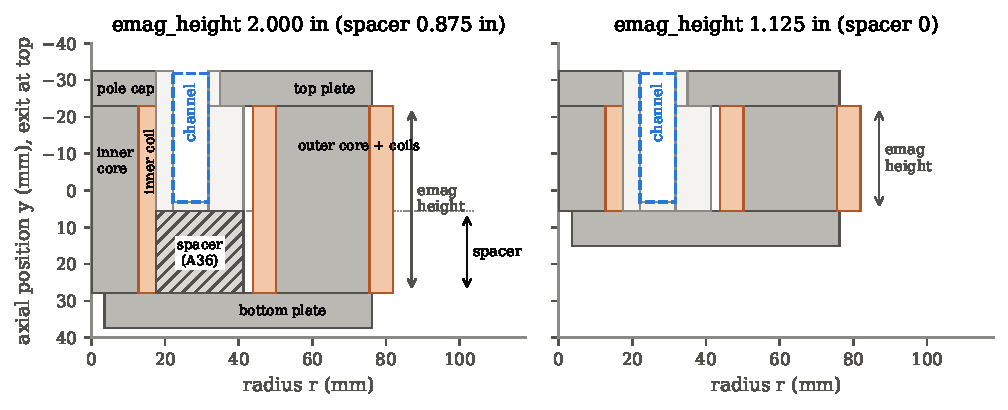
\includegraphics[width=\linewidth]{figures/geometry.pdf}
\caption{Half-section in the plane of one outer core, at the two ends of the sweep. Grey: iron (A36 plates and spacer; A108 cores). Hatched: \texttt{chamber\_spacer}. Orange: windings. Light: chamber (PTFE). Dashed blue: the plasma channel used for every field statistic in this report (r 22.10--31.75~mm, anode at $y=+3.18$~mm, exit at $y=-31.75$~mm).}
\label{fig:geometry}
\end{figure}

Measured directly from the Onshape STEP exports, not assumed:
\begin{itemize}
\item \textbf{The spacer is fixed by \texttt{emag\_height}.} The chamber and top plate never move; the chamber's anode end sits at $y=+5.59$~mm and \texttt{emag\_height} moves only the bottom plate. So
\[ h_\text{spacer} = \texttt{emag\_height} - 1.125~\text{in}, \]
and $h_\text{spacer}\ge 0$ means $\texttt{emag\_height}\ge1.125$~in. At exactly 1.125~in Onshape drops the spacer body and the bottom plate sits on the chamber. All coils and cores are \texttt{emag\_height} tall.
\item \textbf{The inner coil cannot grow outward.} The chamber bore and the spacer bore are both $r=17.46$~mm, exactly the inner coil's outer radius (OD 1.375~in). With the chamber fixed, the inner winding window is $4.76~\text{mm}\times\texttt{emag\_height}$ at the current 1.000~in core. It can only be recovered by thinning the core under the winding (\texttt{inner\_coil\_id}); the pole cap stays at 1.375~in regardless.
\item \textbf{The outer coils have room.} Outer core axes sit 62.86~mm off-axis and the chamber's outer wall is at $r=41.28$~mm, so an outer coil can reach $\approx1.70$~in OD before touching it (currently 1.5~in).
\item \textbf{Stock thicknesses.} The spacer is a single laser-cut A36 part only at a stocked thickness: 0.187, 0.250, 0.313, 0.375 or 0.500~in. Those are marked $^\dagger$ in the tables.
\end{itemize}

\section{Materials}

\begin{table}[htbp]
\centering\small
\begin{tabular}{@{}>{\raggedright}p{3.3cm}>{\raggedright}p{4.3cm}>{\raggedright}p{2.0cm}>{\raggedright\arraybackslash}p{5.2cm}@{}}
\toprule
Part & Material & Source & Magnetic model \\
\midrule
Top, bottom plates; spacer & ASTM A36, hot-rolled P\&O & SendCutSend & AISI 1008 curve as proxy (secondhand) \\
Inner, outer emag cores & ASTM A108 cold-finished bar (taken as 1018) & McMaster & measured 1020 curve, Fermilab TM-1197 \\
Windings & fiberglass-served Cu magnet wire & -- & $\mu_r=1$; current density only \\
Chamber & PTFE & -- & $\mu_r=1$ (not meshed) \\
\bottomrule
\end{tabular}
\caption{Materials. Full properties, sources and confidence ratings are in \texttt{MATERIALS.md}.}
\label{tab:materials}
\end{table}

The circuit is gap-dominated, so the channel field barely depends on the iron grade (Sec.~\ref{sec:method}). Grade does set where a thinned core saturates, which is why the cores are judged against a measured curve (Fig.~\ref{fig:core}, right). Cold drawing lowers permeability slightly relative to the measured stock; a stress-relief anneal after machining recovers it if a core ever runs near the knee.

\section{Method}
\label{sec:method}

\paragraph{Geometry.} Each point is a full-assembly STEP export from the parametrised Onshape document (5 configuration parameters), imported, meshed and solved in 3D by the Gmsh/GetDP pipeline (magnetic vector potential, edge elements, ${\sim}5.9\times10^5$ unknowns). The chamber is fixed, so the channel region is taken from its CAD-confirmed dimensions rather than re-detected per run.

\paragraph{Linear iron, and why that is enough.} Every sweep point uses linear iron ($\mu_r=1500$), about 2.5~min per solve against ${\sim}70$~min nonlinear. Checked, not assumed: on the baseline geometry the linear solve reads \LinVsNLPct\% on the exit field relative to the committed nonlinear (A36-proxy) solve at equal current. A second check re-solved the highest-core-flux geometry (0.750~in core, 0.875~in spacer) with nonlinear iron. Its half-current stage converged (9 Picard iterations), but the full-current stage stalled at a relative residual of 0.11 instead of reaching $10^{-4}$, so \emph{it is not a validated solution}. Taken for what it is, its field agrees with the linear solve to 0.3\% on the exit field and 0.5\% in the outer cores, and puts the inner-core shaft flux density 3.4\% \emph{lower} (the linear figures are conservative there). The one sizeable disagreement is the 99.9th-percentile iron field (13\% higher), i.e. a small number of high-field corner elements, which is plausibly where the Picard iteration is stuck. A finer ramp (nine stages, 50--100\%) was then tried: the 50\%, 60\% and 70\% stages converged (9, 16 and 35 iterations), but Picard contraction fell with every stage (about $2.3\times$, $1.7\times$, $1.2\times$ per iteration) and at 75\% dropped to about $1.1\times$, projecting past the 60-iteration cap, while solver memory grew to 13~GB. It was terminated. The difficulty rises with current level rather than step size, so a converged full-current check needs a Newton iteration, not a finer ramp.
Because the model is linear, each geometry needs one solve: the field scales with ampere-turns, so the A-turns for exactly 300~G at the exit follow by scaling, and so do the iron flux densities.

\paragraph{Excitation.} Inner and outer A-turns are held at the committed ratio (338 : 215 per coil, the field-direction optimum from the earlier current-ratio sweep) and scaled together to put the channel-averaged $B_r$ at the exit station at 300~G. Sweeping the ratio per geometry is a cheap follow-up (two basis solves each) if the shape results below suggest it.

\paragraph{Metrics.} The channel is split into 20 axial stations from anode to exit; $B_r$ and $B_\text{axial}$ are volume-element averages over each station. Radial purity is the mean of $B_r/|B|$. Core flux density is the mean axial $B$ across the shaft cross-section (inside 90\% of the core radius), taken at its maximum along the shaft, since leakage flux joins the core along its length.

\paragraph{Windings.} \texttt{sizing/winding\_design.py} turns A-turns into a winding. Hexagonally nested round wire; insulated diameters are single-glass-served estimates. The inner coil is wound full; the outer coils are wound to whatever turn count gives the required A-turn ratio at the same series current (or full, if the outer window runs out first). Resistance uses the radius the copper actually occupies. It reproduces the committed 260/165-turn AWG~20 design exactly.

\paragraph{Thermal.} \texttt{thermal/radiation\_balance.py}: vacuum, radiation from the outer envelope only (taken from each geometry's own mesh), emissivity 0.30, coils bonded to their cores. Temperatures feed back into copper resistance.

\section{Results}
\label{sec:results}

\subsection{Field in the circuit}
Fig.~\ref{fig:fieldmaps} shows the flux path at both ends of the sweep: up the inner core, radially across the channel from the pole cap to the top-plate bore, down the outer cores and back through the bottom plate. The field in the channel is set by that exit gap, which is identical in every configuration, so the two maps differ mainly behind the channel. With a long spacer, the steel spacer sits just 4.8~mm from the inner core, across the inner winding, and offers flux a path back to the bottom plate that bypasses the channel (this is what loads the core; Sec.~\ref{sec:results}.4). With no spacer, the bottom plate sits 2.4~mm behind the anode face instead.

\begin{figure}[H]
\centering
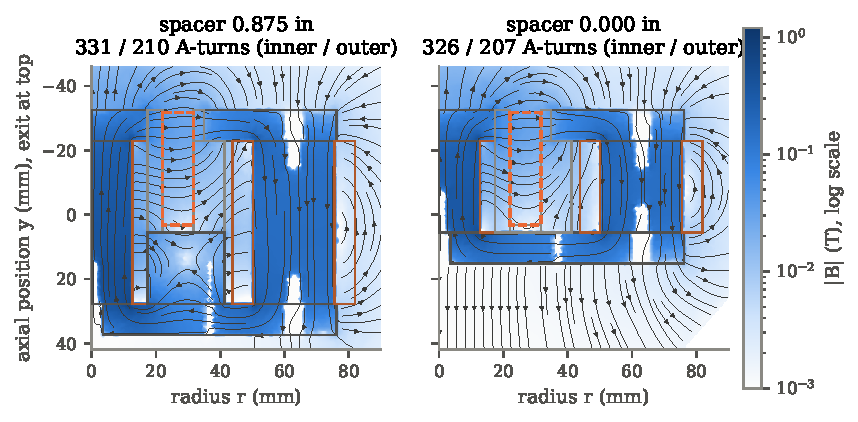
\includegraphics[width=\linewidth]{figures/field_maps.pdf}
\caption{$|B|$ (log scale) and field lines in the plane through the axis and two opposite outer cores, at each geometry's own 300~G excitation, 1.000~in core. Left: longest spacer swept (0.875~in). Right: no spacer. Outlines: iron, windings, chamber; dashed orange: plasma channel.}
\label{fig:fieldmaps}
\end{figure}

\begin{figure}[H]
\centering
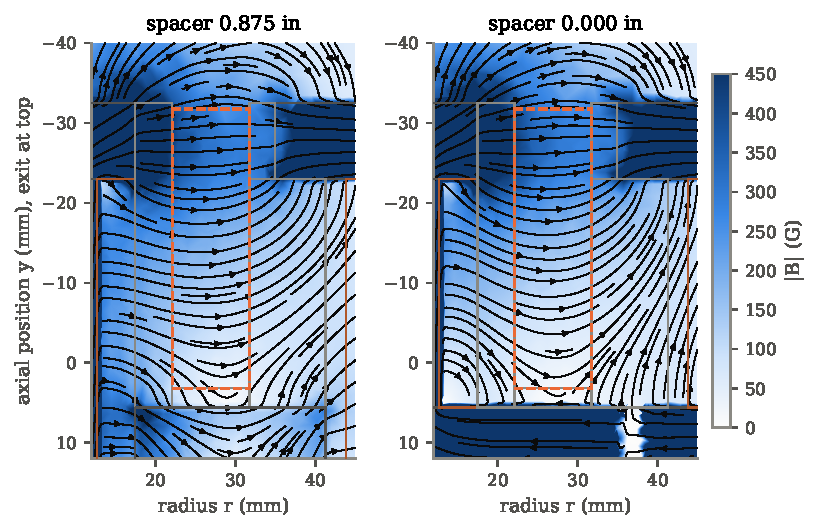
\includegraphics[width=0.92\linewidth]{figures/channel_zoom.pdf}
\caption{Close-up of the channel (dashed), linear colour scale in gauss, same two geometries. The field crosses the channel radially from the inner pole cap to the top-plate bore and weakens toward the anode.}
\label{fig:zoom}
\end{figure}

\subsection{Channel field shape}
Every configuration keeps the same basic lens shape: $B_r$ rises from the anode to a peak of about 317~G roughly 4~mm inside the exit plane, and is 300~G at the exit by construction (Fig.~\ref{fig:profiles}). The spacer only moves the anode half of the profile. Shorter spacers pull the anode-end field down (43~G at 0.875~in to 22~G at 0, 1.000~in core), which moves it toward the target lens and away from the anode, and they reduce the axial component there. The trade is a slightly less radial field overall: radial purity falls from 97.0\% to 95.9\% (Table~\ref{tab:magnetics}). A thinner core shifts the anode field by only a few gauss. All configurations still overshoot the idealised target in the middle of the channel; that is a property of this pole geometry, not of the spacer.

\begin{figure}[H]
\centering
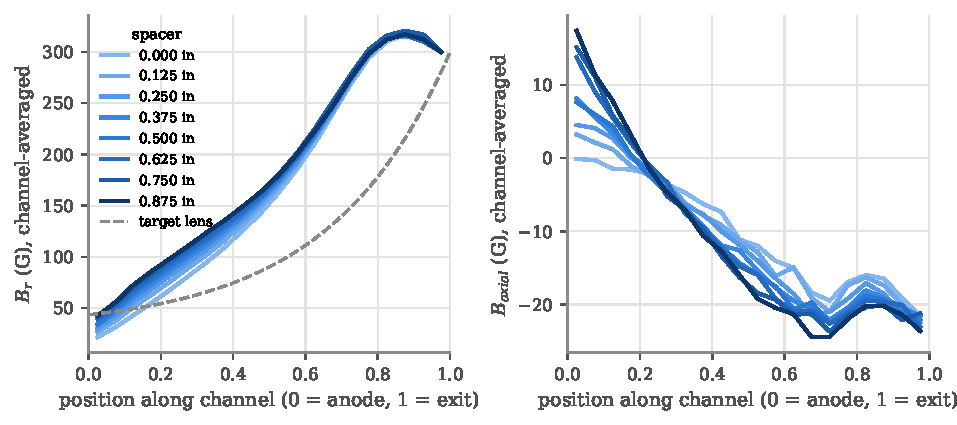
\includegraphics[width=\linewidth]{figures/channel_profiles.pdf}
\caption{Channel-averaged radial (left) and axial (right) field from anode to exit, every spacer height, 1.000~in core, each at its own 300~G excitation. Dashed grey: the target magnetic-lens profile used by \texttt{field\_quality.py}.}
\label{fig:profiles}
\end{figure}

\subsection{Ampere-turns needed}
The A-turns needed for 300~G barely move (Fig.~\ref{fig:at}). Removing the spacer entirely changes the requirement by \AtChangePct\% at the 1.000~in core, comparable to the $\pm1$\% scatter between neighbouring points, which is mesh noise (each geometry is re-meshed from scratch). The one systematic trend is the core: a 0.750~in core needs about 2\% more A-turns than a 1.000~in one, as more of the inner coil's flux leaks past the thinner core. Growing the outer coils to 1.625~in OD (one check point, 1.5~in \texttt{emag\_height}) changes the requirement by \OuterODChangePct\%, i.e. not at all: outer-coil OD is purely a winding-room choice.

\begin{figure}[H]
\centering
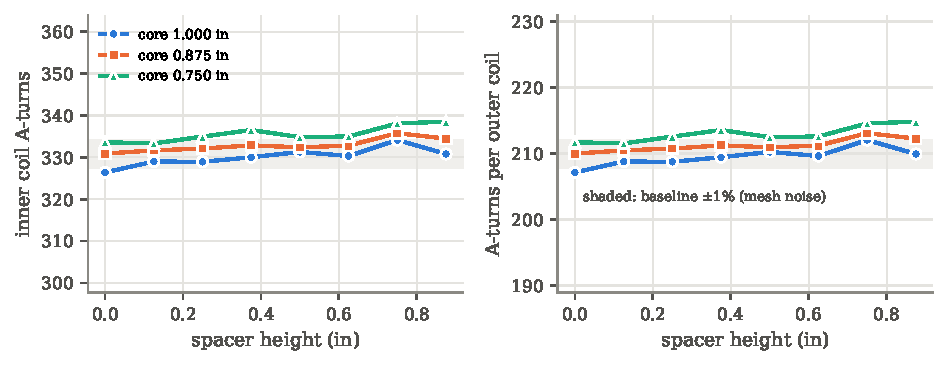
\includegraphics[width=\linewidth]{figures/ampere_turns.pdf}
\caption{A-turns for 300~G at the channel exit, inner coil and each outer coil, and the resulting field per inner ampere-turn.}
\label{fig:at}
\end{figure}

\subsection{Core flux density}
Every core stays far below the knee (Fig.~\ref{fig:core}). The inner core's shaft flux density runs 0.34--0.46~T at 1.000~in, 0.45--0.56~T at 0.875~in and 0.61--0.74~T at 0.750~in, scaling roughly with $1/d^2$ as it must for a fixed flux. The outer cores sit at 0.17--0.19~T throughout. Counter-intuitively, core flux is highest at the \emph{longest} spacer. The steel spacer wraps the inner coil and gives flux a return path through the bottom plate, so the lower part of the core carries that leakage on top of the useful channel flux. Shortening the spacer removes it. The worst case in the sweep, \WorstCoreB~T, is about half the 1.3--1.5~T knee; on the measured 1020 curve the cores stay on the steep, near-linear part of the curve everywhere swept.

\begin{figure}[H]
\centering
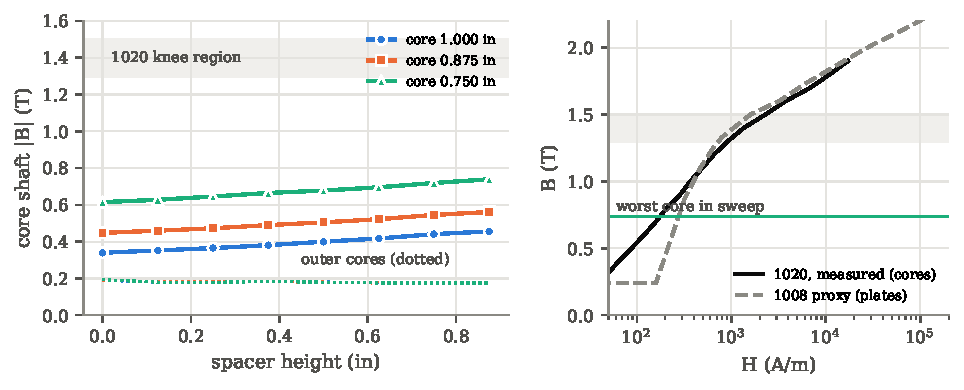
\includegraphics[width=\linewidth]{figures/core_flux.pdf}
\caption{Left: highest shaft-averaged flux density along each core at 300~G, per inner-core diameter (solid: inner core; dotted: outer cores). Right: the measured 1020 curve used for the cores and the 1008 proxy used for the plates, with the worst swept core marked. Shaded: the knee.}
\label{fig:core}
\end{figure}

\subsection{Coil geometries and windings}
Table~\ref{tab:geometry} lists every coil geometry. Tables~\ref{tab:magnetics} and \ref{tab:awg20} give the magnetics and the AWG~20 winding for each; Appendix~A has every gauge.

Three things stand out in Fig.~\ref{fig:winding}:
\begin{itemize}
\item \textbf{Current and power track winding room, not the field.} The A-turns are almost constant, so current is inversely proportional to how many turns fit. The inner window is (core-to-chamber build) $\times$ \texttt{emag\_height}, and both a short spacer and a thick core shrink it.
\item \textbf{String voltage is nearly constant} at 4.0--4.5~V hot across every AWG~20 design. For a fixed gauge $V = IR = (NI)\,\rho\,L_\text{turn}/A_\text{wire}$: it depends only on the A-turns and the mean turn length, not on how many turns fit. Since the A-turns hardly change, neither does the voltage, and power ($VI$) follows current.
\item \textbf{A thinner core offsets a shorter spacer.} Each step from 1.000 to 0.875 to 0.750~in roughly offsets 0.4~in of spacer. No spacer with a 0.750~in core (261/166 turns, 1.28~A, 5.4~W, 69$^\circ$C) matches today's design (260/165 turns, 1.27~A, 5.1~W, 61$^\circ$C) almost exactly.
\end{itemize}
Every configuration is thermally comfortable: the hottest coil is 95$^\circ$C (1.000~in core, no spacer), against a 200$^\circ$C wire-insulation limit.

\begin{table}[htbp]
\centering\small
\begin{tabular}{@{}rrrrrrrrr@{}}
\toprule
spacer & emag\_height & \multicolumn{4}{c}{inner coil} & \multicolumn{3}{c}{outer coil (each)} \\
\cmidrule(lr){3-6}\cmidrule(lr){7-9}
(in) & (in) & ID (in) & OD (in) & build (mm) & window (mm$^2$) & ID (in) & OD (in) & window (mm$^2$) \\
\midrule
\tabinput{generated/tab_geometry.tex}
\bottomrule
\end{tabular}
\caption{Coil geometry of every swept configuration. Inner coil ID = core diameter; OD is fixed at 1.375~in by the chamber bore. $^\dagger$~spacer at a stocked A36 thickness.}
\label{tab:geometry}
\end{table}

\begin{table}[htbp]
\centering\small
\begin{tabular}{@{}rrrrrrrrrr@{}}
\toprule
spacer & core & \multicolumn{2}{c}{A-turns for 300 G} & $B_r$ peak & $B_r$ anode & radial & \multicolumn{2}{c}{shaft $|B|$ (T)} & iron \\
\cmidrule(lr){3-4}\cmidrule(lr){8-9}
(in) & (in) & inner & outer ea. & (G) & (G) & purity (\%) & inner & outer & p99.9 (T) \\
\midrule
\tabinput{generated/tab_magnetics.tex}
\bottomrule
\end{tabular}
\caption{Magnetics per configuration, at each one's 300~G excitation (linear iron).}
\label{tab:magnetics}
\end{table}

\begin{table}[htbp]
\centering\small
\begin{tabular}{@{}rrrrrrrrrrrr@{}}
\toprule
spacer & core & \multicolumn{2}{c}{inner} & \multicolumn{2}{c}{outer (each)} & $I$ & $R_{20}$ & $V_\text{hot}$ & $P_\text{hot}$ & $T_\text{coil}$ & wire \\
\cmidrule(lr){3-4}\cmidrule(lr){5-6}
(in) & (in) & turns & layers & turns & layers & (A) & ($\Omega$) & (V) & (W) & ($^\circ$C) & (m) \\
\midrule
\tabinput{generated/tab_awg20.tex}
\bottomrule
\end{tabular}
\caption{AWG~20 winding for every configuration (the committed gauge), series string of all five coils. Other gauges: Appendix~A.}
\label{tab:awg20}
\end{table}

\begin{figure}[H]
\centering
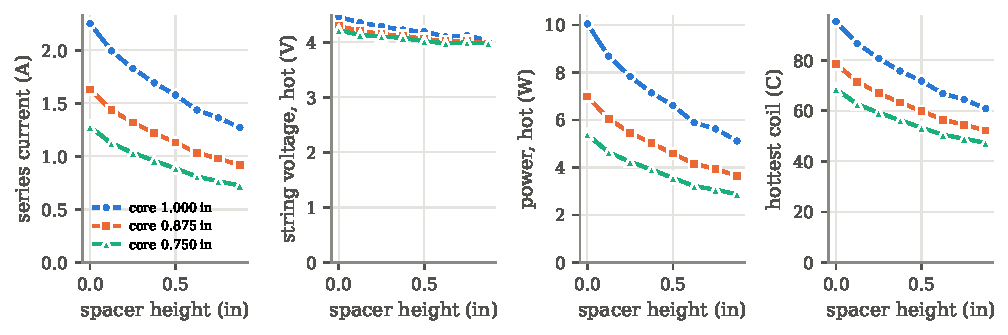
\includegraphics[width=\linewidth]{figures/winding_awg20.pdf}
\caption{AWG~20: series current, string voltage and power at operating temperature, and hottest-coil temperature, per spacer height and core diameter.}
\label{fig:winding}
\end{figure}

\section{Power-supply requirements}
\label{sec:psu}

Nothing in the magnetics depends on the gauge: only the ampere-turn product reaches the field. The gauge sets how that product splits into current and voltage, and therefore which supply fits. Table~\ref{tab:psu} gives, for each gauge, the envelope over \emph{every} swept geometry, so a supply chosen from it covers whichever spacer height is picked. Fig.~\ref{fig:psu} shows the same designs as operating points.

\begin{table}[htbp]
\centering\small
\begin{tabular}{@{}rccccl@{}}
\toprule
AWG & current (A) & max voltage, hot (V) & max power (W) & string $L$ (mH) & suggested supply rating \\
\midrule
\tabinput{generated/tab_psu.tex}
\bottomrule
\end{tabular}
\caption{Supply envelope per wire gauge across all swept geometries (one series string, all five coils). ``Hot'' is at the steady-state coil temperature. Suggested rating: 1.25$\times$ the highest current (room for the linear-model and wire-diameter uncertainty and a field margin above 300~G) and 2$\times$ the highest hot voltage (room for lead resistance and ramping into the inductance).}
\label{tab:psu}
\end{table}

\begin{figure}[H]
\centering
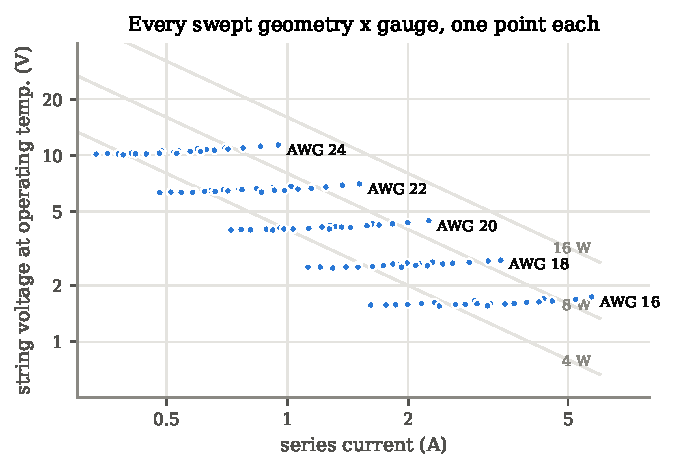
\includegraphics[width=0.62\linewidth]{figures/psu_map.pdf}
\caption{Every swept geometry in every gauge as a (current, voltage) operating point, with lines of constant power. Gauge moves a design along a constant-power line; geometry moves it across the lines.}
\label{fig:psu}
\end{figure}

What the supply needs, independent of gauge:
\begin{itemize}
\item \textbf{Constant-current (CC) regulation.} The field follows current, not voltage; copper resistance rises about 0.4\%/K as the coils warm, so a constant-voltage supply would let the field drift down by the same amount. Any bench supply with a CC mode works; the load is a plain resistor-inductor.
\item \textbf{One channel is enough.} All five coils run in series from one current. The inner/outer ratio is set by turn counts, not by separate supplies. A second supply (or a trim resistor on one leg) is only needed to tune the ratio in the lab.
\item \textbf{Inductance, and switching off.} Stored field energy at the operating point is \StoredEnergyMJ~mJ (from the nonlinear baseline solve), independent of gauge, so the string inductance is $L = 2W/I^2$ (Table~\ref{tab:psu}). Ramp the current up and down rather than stepping it, and put a flyback diode (or TVS) across the string so an open circuit or relay under current cannot generate a large voltage spike. The time constant $L/R$ is tens of milliseconds, so ripple is heavily filtered and does not matter.
\item \textbf{Polarity.} The inner winding is driven opposite to the outer windings (flux crosses the channel from the inner pole to the top plate). Wire the string so the inner coil's sense is reversed relative to the four outer coils, and check it with a gaussmeter at first power-up: wrong polarity collapses the channel field.
\item \textbf{Floating output.} The coils sit next to the discharge; an isolated (floating) output keeps the magnet circuit independent of the discharge supply's reference.
\end{itemize}

\section{Limitations and open items}
\begin{itemize}
\item \textbf{Insulated wire diameters are estimates.} They set turn counts, which can move by 10--20\% with a real datasheet. That moves current and voltage (and the supply choice), not the field and barely the power.
\item \textbf{Linear iron.} Each point is a linear solve. It is checked against a converged nonlinear solve only at the baseline geometry; the worst-case nonlinear check did not converge (Sec.~\ref{sec:method}), though its unconverged field agrees with the linear one in the channel and cores. The plates' B-H curve is a proxy (1008 for A36). The circuit is gap-dominated, so this mostly matters for the core saturation margin, which is judged against the measured 1020 curve.
\item \textbf{Fixed inner/outer A-turn ratio.} Re-optimising the ratio per geometry could recover some field shape at short spacers.
\item \textbf{The 300~G target is not derived} from the plasma requirements (the top-level sizing script assumes 150~G). The results scale linearly: halving the target halves every A-turn and current figure and quarters every power.
\item \textbf{Magnets-only thermal.} No plasma heat load; emissivity 0.30 assumed (\texttt{thermal/README.md} has the sensitivity).
\end{itemize}

\appendix
\section{Every gauge, every geometry}
\small
\begin{longtable}{@{}rrrcrrrrrrr@{}}
\toprule
spacer & core & AWG & turns in/out & $I$ (A) & $R_\text{hot}$ ($\Omega$) & $V_{20}$ & $V_\text{hot}$ & $P_\text{hot}$ (W) & $T_\text{coil}$ ($^\circ$C) & $J$ (A/mm$^2$) \\
(in) & (in) & & & & & (V) & (V) & & & \\
\midrule
\endhead
\tabinput{generated/tab_all_gauges.tex}
\bottomrule
\end{longtable}
\normalsize

\section{Reproducing this report}
From the repository root:
\begin{verbatim}
cd gmsh_getdp/assembly
python emag_sweep.py --validate            # linear vs committed nonlinear, baseline
python emag_sweep.py                       # full grid, resumable (~1 h)
python emag_sweep.py --nonlinear h1.125_ci0.750_oo1.500
cd ../..
python report/render_3d.py
python report/make_report.py               # figures, tables, PDF (needs tools/tectonic)
\end{verbatim}


\end{document}
